\PlateHeader{Plate 29 --- Guarded Fixed-Point Loop}{Ch. 12}
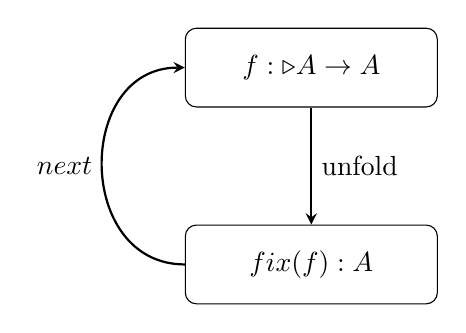
\begin{tikzpicture}[>=stealth]
  \node[draw,rounded corners,minimum width=3.2cm,minimum height=1.0cm] (f) at (0,2.5) {$f:\triangleright A\to A$};
  \node[draw,rounded corners,minimum width=3.2cm,minimum height=1.0cm] (x) at (0,0) {$\operatorname{fix}(f):A$};
  \draw[->,thick] (f)--(x) node[midway,right] {unfold};
  \draw[->,thick] (x.west) .. controls (-3,0) and (-3,2.5) .. (f.west) node[midway,left] {$\operatorname{next}$};
\end{tikzpicture}
